\section{Modelling with UML}
\subsection{Software architecture}
\subsubsection{Component segmentation and description of interfaces}
The purpose of the following diagram is to show the structural relationship between the components of the memory stack, to provide a high-level architectural view and to give a rough information about the components.\\
\begin{center}
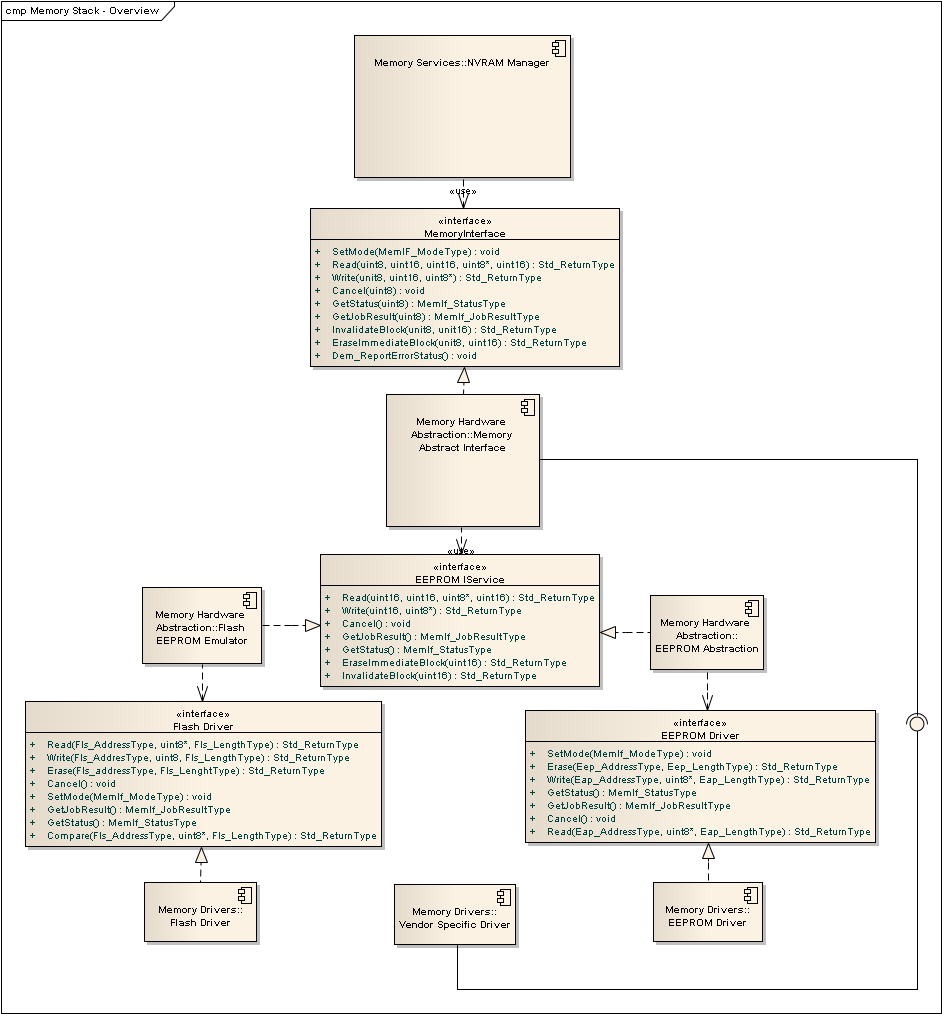
\includegraphics[scale=0.45]{Images/Memory_Stack_Overview_UML.png}
\end{center}
The NVRAM component contains of two main components. They shall provides specific services according to their individual requirements. In particular there is a data management and a maintenance component. The maintenance component is responsible for all loading,writting and saving processes. The data management component is responsible for maintaining  of the non-volite data.
\newline
The Abstract memory Interface
\newline
Flash EEPROM
\newline
EEPROM Abstract
\newline 
FLASH Driver
\newline
EEPROM Driver

\subsubsection{Hardware/Software mapping}
\subsubsection{Management of persistent data}
\subsubsection{Access rights and access control}
\subsubsection{Global control flow}
\subsubsection{Tools}
\subsubsection{Reference}
